\pdfoutput=1

\documentclass{l4proj}

%
% put any packages here
%

\usepackage[]{algorithm2e}
\usepackage{graphicx}
\usepackage{tabularx}

\graphicspath{ {images/} }

\begin{document}
\title{Who's There? Occupancy Prediction with Smart Sensor Boxes}
\author{Jamie Sweeney}
\date{September 26, 2017}
\maketitle

\begin{abstract}
We show how to produce a level 4 project report using latex and pdflatex using the 
style file l4proj.cls
\end{abstract}

\educationalconsent
%
%NOTE: if you include the educationalconsent (above) and your project is graded an A then
%      it may be entered in the CS Hall of Fame
%
\tableofcontents
%==============================================================================



%==============================================================================
%==============================================================================
%==============================================================================
\chapter{Introduction}
\pagenumbering{arabic}


\section{Context}
The “Internet of Things”, or IoT is a term used to describe the expanding network of devices of many types,  ranging from supercomputers to household appliances that contain embedded computer systems, making them capable of communication with other IoT devices. These devices aim to bring technology to every corner of our lives, bringing the idea of interconnected smart homes, workplaces, cities and more to reality.

Since the term was first used in 1999\cite{c-iot-term} the IoT has come a long way,  with the number of internet connected devices rapidly increasing\cite{c-devices}, and although nobody seems to agree on global market predictions, many predict massive growth\cite{c-iot-market1}\cite{c-iot-market2}\cite{c-iot-market3}.

One key area of study has been developing occupancy detection systems that would allow IoT devices to be more aware of the occupancy status of their surroundings. This is a crucial step to implementing smart homes, workplaces and campuses that are responsive and can meet their demands at any given time.

Advanced examples of this are already taking concrete form, with the University of Glasgow investing €1bn towards developing a smart campus\cite{c-iot-uog} and the city of Barcelona making major overhauls to many public services in an attempt to bring the idea of a smart city to reality\cite{c-iot-bar}.



\section{Motivations}
The motivations for this project are wide, with smart sensors being applicable in a broad variety of ways. We will discuss the primary motivations for this project, which are understandably more relatable and accessible to myself, in addition to a number of secondary motivations that are considered due to close similarity.

\subsection{Primary Motivation}
To narrow our field of focus, we choose a main motivation to consider when producing the smart sensor boxes. We consider the following scenario: University administration decide they wish to upgrade buildings with ‘smart sensor boxes’ with the overall goal being that students or other staff members can find occupancy information on certain areas remotely. For example library group study areas could be listed online with an indication of their current use, allowing students who plan on visiting to check availability beforehand.
The University of Glasgow library currently provides a similar feature, displaying computer use breakdown by floor, available from monitors within the library.

In addition the system should be built to be easily extendable, and capable of operating as a part of a larger IoT network. This is critical as there are many potential uses for such a system operating on a larger network of IoT devices. One example would be querying the system for occupancy information on a room and adjusting ventilation and heating based on the number of occupants, a effective system would bring potential for large savings in electricity and heating \cite{c-heating} while requiring very little human intervention or overhead costs.

\subsection{Secondary Motivations}
Although we focus on a university implementation of occupancy prediction, we can imagine a similar design could be incorporated into many different areas. Schools, workplaces and public buildings could all benefit from installing smart sensor functionality, allowing not only occupancy information to end users, but also providing more in-depth analysis of overall occupation to any interested administrators.

For example, smart public buildings could allow local councils to analyse the usage of various public services, allowing them to make more informed decisions on funding, maintenance, staffing and other key elements of operation.

To list a few more: Security systems, home-automation, public transport, gyms, dining locations and other areas of leisure. We can see that this problem is applicable to many areas of life and has the potential to shape cities and communites by providing accurate and reliable information that is used network-wide by many parties.


\section{Goals}
In short, the aim of this project is to design and construct low budget ‘smart sensor boxes’, capable of predicting human occupation in a room. To do this we use the popular brand of microprocessors ‘Raspberry Pis’ in addition to a variety of sensors and other techniques.

In addition to the smart sensor boxes, we will design and implement a centralised hub capable of receiving, storing and serving information produced by a series of RPi boxes. This hub should also provide functionality for system-wide maintenance and configuration, to make setup and operation efficient and flexible.

This system should be built to be easily extendable, and capable of operating as part of the IoT network. This is critical as there are many potential uses for such a system operating on a larger network of IoT devices. 

%==============================================================================
%==============================================================================
%==============================================================================

\chapter{Background Analysis}
We start by researching and reviewing past studies conducted in similar fields, given that the subject matter is broad and widely applicable, we find many studies available. Many employ sensors and machine learning techniques to achieve meaningful results.


\section{Human Detection}
Sensors are a key element in almost every real-world computing application, especially those concerned with the detection of humans e.g automatic doors. Without them a computing device would have little to no information on its surroundings, and would be extremely ineffective for real-time interactive functionality. For this reason, sensors will be a primary component of the smart boxes.

Background research on previously conducted studies gives us a comprehensive list of applicable sensor, and their specific advantages and disadvantages.

\subsection{Infrared Light}
Infrared light is the electromagnetic radiation emitted by all objects with a temperature above 0°K, giving the feeling of heat. The wavelength of IR light spans from 700 nm to 1 mm, existing just outside of the range of human vision\cite{c-inred}. PIR sensors feature a “sensor face” that can detect a change in the average amount of IR light hitting the surface, the sensor then outputs a signal indicating this change, with a low voltage indicating low change, and a higher voltage indicating a greater change\cite{c-pir}.

They are most commonly used in PIR-based motion detectors such as automatic lighting systems. Generally the purpose of a PIR sensor is to detect the presence of humans at a binary level i.e true or false. However it has been shown that with suitable positioning and utilisation of machine learning techniques, a single PIR sensor can be used to predict the number of occupants in a room within a small range to fair accuracy\cite{c-pir-study}.

There are many problems to overcome when using a PIR sensor for this purpose, most importantly, the positioning of the sensor; PIR sensors are prone to interference from occluding objects i.e blocking one another from the sensor. As a result of this, the most ideal position would be the ceiling of the room, however this may not prove as practical for other aspects such as maintenance\cite{c-pir-study}.

Although it will be difficult to obtain a precise estimation by a PIR sensor alone, with the correct implementation, the sensor could potentially be used alongside other components to achieve a valid predictions.

\subsection{Digital Images}
The field of computer vision first emerged in the 1960s and has been developing steadily ever since with large abouts of research being done for a number of different problems. With endless applications from manufacturing to self-driving vehicles, it’s not surprising that there is a variety of methods available to us, specifically much research has been done on object detection and recognition. 

Primitive solutions to object detection might include matching edges from input imagery to predefined templates or a taking and analysing a histogram of oriented gradients (HOG). 

In recent years, more complex designs have been produced, often in combination with machine learning algorithms and a training dataset which has been shown to be effective in a variety of object detection problem areas. 

Although more complex techniques are tempting, it is important to bear in mind the technical restraints put in place by using a microcontroller; computer vision techniques are notorious for being process intentensive and many require the use of optimised graphical processors to achieve realistic processing times. Fortunately modern digital cameras are extremely advanced and cheap, high quality and compatible digital cameras are readily available, specifically the Raspberry Pi 3 Model B+ features a CSI camera port and a separate camera module. The camera module costs around £20, has an 8-megapixel sensor and is capable of recording in 1080p30 and 720p60\cite{c-picamera} which is most definetely enough for our needs.

To conclude, it seems that computer vision could play a vital role in the final design and is definetely due consideration.

\subsection{Audio}

As humans, audio plays a crutial role in understanding our evironment and communicating with each another, as a result we are able to detect human voices with almost absolute certainty. This close relationship suggests that it is a promising area of study in relation to human detection, i.e we use it sucessfully, therefore machine may be able to do the same. 

We find that this is not quite as promising as previously thought, although a fair amount of research has been done on audio analyis by machine for high level tasks such as human detection, we have yet to see an implementation that can perform anywhere near the level of humans for such tasks. Most sucessful applications of audio analysis have been in speech recognition, for example speech to text functionality which has impoved the accessability of many computer systems and applications.

We find that there a few key problems facing predicting human occupancy using audio, one of them being the fact that noise the environment is constantly disturbing audio detections with noise, from a variety of sources. Much progress has been made over the past few decades concerning the analysis of a single human voice, however little has been made in developing to solutions that would be applicable to mass human detection.

Although audio analyis clearly has the potential to be a major componenet in a smart sensor boxes, our findings suggest that the field needs a lot more development before audio analysis can give meaninful occupancy predictions.

\subsection{Other}
\subsubsection{Luminosity}
Luminosity sensors contain photodiodes which convert light to electric energy, allowing them to effectively measure the lighting level of there surrounding. The typical luminosity range of an office or classroom is between 0 and 500 lux, which is well within the standard sensor range of 0 to 40,000 lux . A commonplace example of an application of these sensors would be street lights which turn on and off. Not much information could be found on cases of luminosity sensors being used for human occupancy prediction, but we find that a cheap and easily available luminosity sensor would be able to provide an indication of occupancy, as a dark room would suggest that there are no occupants. We must also consider the possible interferences that may affect the luminosity of the room, or the reading produced by the sensor. Sunlight shining through a window onto the sensor would greatly increase its reading, and could give an inaccurate reading of the room lighting as a whole.
\subsubsection{Temperature}
Another sign of human occupancy could be room temperature, as occupants naturally heat the air through emission of body heat. However the standard precision of an appropriate temperature sensor is usually 0.5°C, which it too low to be useful in determining exact temperature reading. The temperature change undergone when a group of people enter the room is unlikely be high enough to be properly detected by the sensor and be a guaranteed indication of human occupancy. This is especially true when the room temperature is subject to external factors, for example sun shining through the window will cause the room temperature to increase rapidly. We find that it would be too difficult to separate such an event from temperature rises that indicate human activity, so it follows that temperature sensors would be of little use for this problem.
\subsubsection{CO2 and humidity}
In an unregulated air system, human occupants would also give rise to CO2 and humidity levels through breathing, a higher number of occupants would see that the change in CO2 and humidity would be faster meaning the rate of change could give us a fairly accurate prediction. However for this very reason, building air must be properly regulated to ensure that it is safe for human occupancy, therefore any measurements we took would be expected to be within a fairly small range and would be highly influenced by external factors such as air conditioning, open windows and air flows.


\section{Device Detection}
Although the aim of this system is to detect human occupancy, everyday more and more people are using smartphones or similar electronic wireless devices for almost every aspect of life. It is estimted that 81\% of adults in the UK own a smartphone (as of 2016)\cite{c-phones}, and with most of these people using their devices everywhere they go, it is reasonable to say that the number of wireless devices in a specific area would be very highly correlated with the number of human occupants. We must also consider the possibility of rooms containing wireless devices that are not relative to the human occupants, for example lab computers may contain Bluetooth functionality that would distort the human to device ratio, however typical workplace machines operate using wired communication, as it is more practical for a stationary machine.

Over the years, smartphone development has brought about faster and more robust wireless protocols and methods. Since many of these protocols are the same ones used by microcontrollers, it is reasonable to think we may also be able to get an estimation of wireless devices nearby using similar techniques to human detection.

Although this system would greatly benifit from being able to detect all devices in the nearby area, obviously this is not technically feasible with any device, since many users would choose to not broadcast their devices and many protocols are not built with device broadcasting in mind, for example communicating on 3G will not let all other nearby 3G devices know the location such as bluetooth communication might.

The only feasible device detection method we can see is using Bluetooth and Bluetooth Low Energy device scanning, which will recieve alerts from nearby devices that have broadcasting enabled. Although not every bluetooth device will broadcast it's location in response to a device scan, the ratio of devices that respond should be relatively constant for similar audiences. 
 

\section{Exitsting products}
During our background analysis we find that similar systems have been implemented before for real-world production use.

"Meshlium", a product of the IoT provider Libelium, attempts to detect WiFi and Bluetooth communications in the nearby area to obtain a number of devices. It is estimated to detect up to 95\% of nearby wireless devices operating on these protocols\cite{c-meshlium}.

Another IoT solutions provider "Retail Sensing" have developed a CCTV based people counting system which utilises computer vision techniques with CCTV cameras recordings from cities, shopping centres etc. to predict human occupancy by area to up to 98\%\cite{c-sensing}.

Unfortunatelty since these systems are a product costing money, the intellectual propery is protected and technical specifications are vague and mostly refer to "our processing algorithms". However we can at least see that these products are feasible and obtain a general overview of how they work which will be a useful reference during the design stage.

%==============================================================================%==============================================================================
%==============================================================================


\chapter{Requirements}

\section{Functional Requirements}

We begin by defining 6 functional requirements (A-F) for the final system and their associated sub-requirements. The order of requirments should give an indication of the data flow, starting at the sensors and ending with the end user.

\subsection{Sensor data collection (A)}
The smart sensor boxes should be capable of collecting data from connected sensors for a specified period of time. The connected sensors we should support are:
\begin{enumerate}
  \item Bluetooth device scanning.
  \item Bluetooth Low Energy device scanning.
  \item Camera (still images)
\end{enumerate}

\subsection{Sensor data processing (B)}
In addition to data collection, the smart sensor boxes should be capable of performing some form of post-processing on the sensor data. For each implemented sensor, we choose an appropriate processing technique that can be applied:

\begin{enumerate}
  \item Bluetooth and Bluetooth LE devices.
  \begin{enumerate}
    \item Log any bluetooth reponses received to file.
    \item Anonymise device addresses for ethical reasons (only if required).
    \item Collate results from both sensors.
    \item Remove duplicate results where possible.
    \item Retain results for a given period after detection.
    \item Attempt to smooth out connection strength values for each device.
  \end{enumerate}
  \item Images
  \begin{enumerate}
    \item Log any images taken to file.
    \item Apply an object recognition algorithm to the still image.
    \item Log any object recognition output images to file.
    \item Parse output for number of humans found.
  \end{enumerate}
\end{enumerate}

\subsection{Reporting (C)}
The smart sensor boxes should be able to:
\begin{enumerate}
  \item Smooth the output of camera post-processing results to obtain an more reliable metric for a given time.
  \item Collect all devices from device post-processing that are still valid (within decay time range).
  \item Compile a report from: the smoothed people number, the number of devices, the current time, any report meta-data required.
  \item Send this report securely to an external component for furthur use.
  \item Log any reports that are given to file.
\end{enumerate}

\subsection{Data storage (D)}
The system must be capable of storing data about: 
\begin{enumerate}
  \item Buildings, floors, rooms.
\begin{enumerate}
  \item Name.
  \item Description.
\end{enumerate}
  \item Smart boxes.
\begin{enumerate}
  \item Name.
  \item Description.
  \item Location.
  \item Authentication data.
\end{enumerate}
  \item Sensor output.
\begin{enumerate}  
  \item Time.
  \item Sensor reading.
\end{enumerate}
  \item Smart box reports.
\begin{enumerate} 
  \item Time.
  \item Sensor reading.
\end{enumerate}
  \item Estimations.
\begin{enumerate} 
  \item Time.
  \item Location.
  \item Estimate.
\end{enumerate}
  \item Manual readings
\begin{enumerate} 
  \item Time frame.
  \item Location.
  \item Reading.
\end{enumerate}
  \item Admin users.
\begin{enumerate} 
  \item Username.
  \item Hashed password (it is unsecure to store plain passwords for many reasons).
\end{enumerate}
\end{enumerate}

\subsection{Estimating occupancy (E)}
The system should be able to use smart box reports, to give an estimation of occupancy for each location with reports.
\begin{enumerate}
  \item Generate some form of regression model for each sensor type.
  \item Train each model using a combination of smart box reports values and true readings for the associated room and time range.
  \item We should be able to continue to train the models on and off, so they can continually improve throughout service.
  \item Use new reports to generate occupancy estimates using an average of all recent report data for each smart sensor box.
  \item The system should be capable of making estimated with missing report values to ensure that not all sensors are essential for every smart box node.
  \item The system should also be able to use reports from multiple smart sensor boxes in the same area, and take an average of the seperate estimations.
\end{enumerate}

\subsection{Data serving (F)}
\begin{enumerate} 
  \item We should provide public available REST API endpoints that allow access to data on:
  \begin{enumerate}
    \item Buildings.
    \item Floors.
    \item Rooms.
    \item Room estimates.
  \end{enumerate}
  \item We should provide private (user only) available REST API endpoints that allow addition, removal and modifcation of data on:
  \begin{enumerate}
    \item Buildings.
    \item Floors.
    \item Rooms.
    \item Smart boxes.
    \item Users.
  \end{enumerate}
 \item We should provide a front-end display that provides an interface for the public api to end users.
 \item We should also provide a front-end display that provides an interface for the private api.
\end{enumerate}

\section{Non-functional Requirements}
For each functional requirement we also state several non-functional requirments that are still essential to an effective solution.

\subsection{Sensor data collection (A)}
\begin{itemize}
  \item Ideally each smart sensor box should be as cheap as possible while providing adequte data, in order for the system to be scaled up without large overhead costs.
  \item If the data cannot be collected continuously, meaning they require some amount of time to compute results before obtaining a new reading, then we should perform as many iterations as possible to ensure that results are up to date.
  \item The data collection should be able to run for as long as possible without human intervention to reduce the amount of maintainence required.
\end{itemize}


\subsection{Sensor data processing (B)}
\begin{itemize}
  \item The post processing should be as quick as possible to ensure that final reports are not heavily delayed.
  \item The processing required should be as light as possible, as the Raspberry Pi does not have a large processing capacity. We should also seek to use optimised processing implementations where possible.
\end{itemize}

\subsection{Reporting (C)}
\begin{itemize}	
  \item To ensure that occupancy reports and predictions are not outdated, RPis should be able to send reports at a rate of atleast one report per minute. The reports should also stick to the specified rate with fair accuracy and not deviate too far from a steady report rate.
  \item Extensibility - the report formatting should take a standard form such as JSON and be easily extendible to allow the use of more sensors.
\end{itemize}

\subsection{Data storage (D)}
Any data stored should be:
\begin{itemize}	
  \item Implemented in an efficient and correct manner, without unnecessary dependencies between data.
  \item Scalable without any major modifications.
  \item Accessible as quickly as possible and with no down-time.
  \item Secure from malicious attack or unauthorised access.
\end{itemize}


\subsection{Estimating occupancy (E)}
\begin{itemize}	
  \item The estimates should be as accurate as possible.
  \item Estimates should be produced at a reasonable enough rate to ensure that they are not out of date.
\end{itemize}


\subsection{Data serving (F)}
Any data stored should be:
\begin{itemize}	
  \item User friendly and easy to use.
  \item As up to date as possible.
\end{itemize}


%==============================================================================
%==============================================================================
%==============================================================================
\chapter{Design}
\section{High Level Summary}

We start by splitting the requirements to three seperate components with individual functions.
\begin{enumerate}
  \item Smart Sensor Boxes:
	Collects data from the various sensors, also generate reports detailing RPi identification, allong with smoothed sensor data. Reports are then sent to the HTTP server for analysis. 
  \item Centralised Storage:
	A database that allows for the storing and querying of data must contain information on building, RPis, estimates, reports, users etc.
  \item HTTP Server:
	A simple HTTP application that can receive sensor report data from the smart sensor boxes. The sever should also be able to perform estimations for locations based on reports and also feature a web application that serves this data to the users. 
\end{enumerate}
Figure \ref{fig:overalldiag} Shows a simple high level diagram of the system design.
%=========
\begin{figure}
\centering
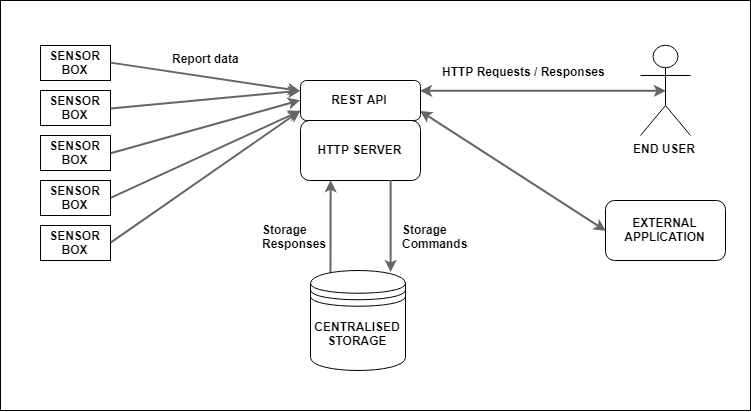
\includegraphics[width=\textwidth]{overalldiag}
\caption{High level design of system.}
\label{fig:overalldiag}
\end{figure}
%=========


\section{Smart Sensor Boxes (A-C)}
The smart sensor box logic consist of a main reporter algorithm which initialises scanning for each detection method and monitors the output. Every time a report is required, the algorithm takes the outputs from each output queue, and collates them to a report which is sent to the HTTP server for furthur use.  Algorithm \ref{RPA} shows the pseudocode for this algorithm.
%=========
\begin{figure}
\centering
\includegraphics[width=\textwidth]{rpidiag}
\caption{High level diagram of the smart sensor box implementation.}
\label{fig:rpidiag}
\end{figure}
%=========


The detection methods supported are:
\begin{enumerate}
  \item Bluetooth / BTLE device scanning - Continuously scans for devices and adds any discoveries to a output map, scans are done for a specified time before restarting to ensure that devices do not stop responding the the scan signal. Algorithm \ref{BTS} details the algorithms used.
  \item Camera and object detection - Runs on a loop taking images and feeding them into an object detection algorithm which predicts objects and their certainty. The number of people is extracted from the detection output and smoothed with previous results using an average of the previous value and the new prediction. Algorithm \ref{CMS} details the algorithms used.
\end{enumerate}
%=========
\begin{algorithm}
\DontPrintSemicolon
\nl $\textbf{void}~scanBluetooth(\textbf{Int}~T_{cycle}, \textbf{Int}~T_{timeout}, \textbf{Int}~T_{decay}, \textbf{Map}~output)$ \;
\nl \Begin{
\nl \While {$T_{timeout} > T_{now}$}{
\nl $scan(T_{cycle}, T_{decay})$\;
\nl \While {$scanning$}{
\nl $discovery \gets new\textunderscore discovery$\;
\nl $handleDiscovery(T_{decay}, discovery, output)$\;
}
}
}
\;
\nl $\textbf{void}~handleDiscovery(\textbf{Int}~T_{decay}, \textbf{Map}~discovery, \textbf{Map}~output)$ \;
\nl \Begin{
\nl $addr \gets discovery['address']$\;
\nl $rssi \gets discovery['rssi']$\;
\nl $time \gets discovery['time']$\;
\nl \eIf {$address\ in\ output$}{
\nl $old \gets output[addr]$\;
\nl \eIf {$old['time'] + T_{decay} < T_{now} $}{
\nl $new \gets \{'rssi': (rssi + old['rssi'])/2, 'time': time\}$\;
\nl $output[addr] \gets new$\;
\nl }{
\nl $new \gets \{'rssi': rssi, 'time': time\}$\;
\nl $output[addr] \gets new$\;
}
}{
\nl $new \gets \{'rssi': rssi, 'time': time\}$\;
\nl $output[addr] \gets new$\;
}
}
\;
\caption{Pseudocode for Bluetooth and Bluetooth Low Energy device scanners.}
\label{BTS}
\end{algorithm}
%=========

%=========
\begin{algorithm}
\DontPrintSemicolon
\nl $\textbf{void}~scanCamera(\textbf{Int}~T_{cycle}, \textbf{Int}~T_{timeout}, \textbf{Int}~output)$ \;
\nl \Begin{
\nl \While {$T_{timeout} > T_{now}$}{
\nl $img \gets takeImage()$\;
\nl $objs \gets objectDetection(img)$\;
\nl $hum \gets numHuman(objs)$\;
\nl $output \gets (output + hum)/2$\;
\nl $wait(T_{cycle})$\;
}
}
\;
\caption{Pseudocode for the camera detection algorithm.}
\label{CMS}
\end{algorithm}
%=========


%=========
\begin{algorithm}
\DontPrintSemicolon
\nl $\textbf{void}~reporter(\textbf{Int}~T_{cycle}, \textbf{Int}~T_{timeout})$ \;
\nl \Begin{
\nl $T_{decay}, T_{ccycle}, T_{bcycle} \gets getConfig()$\;
\nl $auth \gets getAuthData()$\;
\nl $bt\textunderscore output \gets new\ \textbf{Map}$\;
\nl $cm\textunderscore output \gets 0$\;
\nl $scanBluetooth(T_{bcycle}, T_{timeout}, T_{decay},bt\textunderscore output)$\;
\nl $scanCamera(T_{ccycle},T_{timeout}, cm\textunderscore output)$\;
\nl \While {$T_{timeout} > T_{now}$}{
\nl $devices \gets bt\textunderscore output$\;
\nl $people \gets cm\textunderscore output$\;
\nl $report \gets \{ 'devices':devices, 'people':people, 'time': T_{now}, 'auth': auth\}$\;
\nl $sendReport(report)$\;
\nl $wait(T_{cycle})$\;
}
}
\;
\caption{Pseudocode for the reporter algorithm.}
\label{RPA}
\end{algorithm}
%=========

\section{Centralised Storage (D)}
The centralised storage component should take the form of a database. We start by defining the entities as:

\begin{itemize}	
  \item Building
  \item Floor
  \item Room
  \item Rpi
  \item Report
  \item Estimate
  \item Reading
  \item User
\end{itemize}

In addition to the data fields set out in the requirements stage, we must use foreign keys to map out the relationships between these entities:
\begin{itemize}
  \item Buildings may contain one or more floors.
  \item Floors may contain one or more rooms.	
  \item Rooms may contain one or more RPis.
  \item RPis may produce one or more reports.
  \item An estimate has one associated room, and room may have one or more estimates.
  \item An reading has one associated room, and room may have one or more reading.
\end{itemize}

To ensure that each entity instance can be uniquely identified, the database should store an associated integer id for each table row.
We must also store an authorisation key for each smart sensor box, that will allow the server to verify the validity of any incoming reports.
It is also important to note that when storing passwords we should hash them beforehand, this ensures that passwords are not compromised, while still allowing us to verify user logins.

Figure \ref{fig:ERdiagram} Shows an ER diagram of database design.
%=========
\begin{figure}
\centering
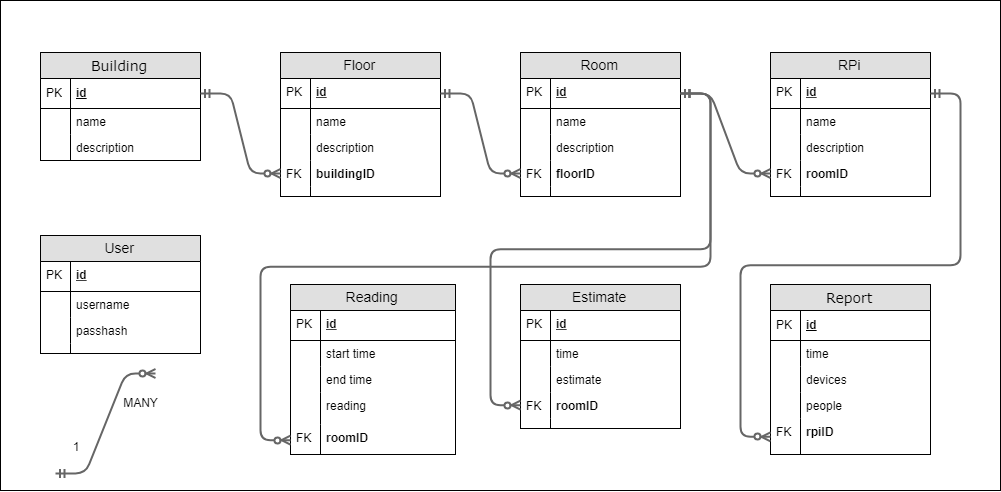
\includegraphics[width=\textwidth]{ERdiagram}
\caption{ER diagram of database design.}
\label{fig:ERdiagram}
\end{figure}
%=========



\section{HTTP Server (E-F)}

Server design is fairly boilerplate, the only notable design choices are concerning the webpage design and the prediction model.

We set out the pseudocode for performing tasks relating to estimation and predictions.

Additionally we provide wireframes to base the final web pages on. We design a simple page for each of the public pages: home, building page, floor page and room page. The page title is left blank for now, but should be replaced with a suitable title e.g "Room Occupancy Viewer".

Figure \ref{fig:homewireframe}, Figure \ref{fig:buildingwireframe}, Figure \ref{fig:floorwireframe} and Figure \ref{fig:roomwireframe} show these wireframe designs. The header buttons will allow the user to navigate between pages, in addition clicking on a building, floor or room should take the user to the page for that entitiy. For further clarification, the final wireframe depicts a room page, consisting of a small information box and a line graph showing the estimate over time.

%=========
\begin{figure}
\centering
\includegraphics[width=\textwidth]{homewireframe}
\caption{Home page wireframe.}
\label{fig:homewireframe}
\end{figure}
%=========
%=========
\begin{figure}
\centering
\includegraphics[width=\textwidth]{buildingwireframe}
\caption{Building page wireframe.}
\label{fig:buildingwireframe}
\end{figure}
%=========
%=========
\begin{figure}
\centering
\includegraphics[width=\textwidth]{floorwireframe}
\caption{Floor page wireframe.}
\label{fig:floorwireframe}
\end{figure}
%=========
%=========
\begin{figure}
\centering
\includegraphics[width=\textwidth]{roomwireframe}
\caption{Room page wireframe.}
\label{fig:roomwireframe}
\end{figure}
%=========














%==============================================================================
%==============================================================================
%==============================================================================

\chapter{Implementation}
The system was implemented using as many extenal libraries as possible, in order to reduce the code required and time taken to develop. A private Github repository was used to manage versions, in addition we use the default Github ticket management service to organise the workload and document progress. We use 3 milestones to seperate the tasks by priority, low priority tasks are assigned to milestone 'Minor', wheras higher priority tasks get assigned to 'Urgent', the lowest priority is 'Backlog' which holds tasks that likely will not get completed due to time restraints. We also use the convenient Github wiki service which allows us to document  everything along with source code. We attempt to document as much as possible during implemation as this is a crucial step in producing a realistically usable software product. 

\section{Smart Sensor Boxes (A-C)}
The smart sensor boxes were implemented using the popular brand of microprocessors “Raspberry Pi”, the RPis were a great choice for a smart sensor box such as this due to the fact that it is compatible with a wide variety of sensors and have relatively powerful computation ability. Specifically we use the most recent version, “Raspberry Pi 3 Model B” which features inbuilt WiFi and Bluetooth adapters, as well as a dedicated RPi camera port.

\subsection{Sensor data collection}
Since the RPi 3B has an inbuilt Bluetooth adapter, we can use the Python module “bluez” to constantly perform a scan for nearby Bluetooth devices that are broadcasting nearby. We find an example Python script with similar desired functionality, we modified this file by adding a 'start' function that other Python modules can call with an output queue. Similarly, we use the module “bluepy” to scan for Bluetooth Low Energy devices, implementation is relatively simple, we perform a standard BTLE scan with a custom class to handle devices, which are sent to the BTLE output queue. 

We collect still images from the camera module using the Python module "picamera" which provides a Python interface for the Raspberry Pi camera module. Obtaining an image is as simple as a function call, with a filename as argument.


\subsection{Sensor data processing}
To process all Bluetooth and BTLE devices, we create a thread-safe dictionary object that holds device infomation as value, with device address as the key. When we perform device scanning, we pass a seperate output queue to each device scanner and periodically check for new additions, these additions are taken from the que and inserted to the dictionary using a custom 'add' method.

Captured image files are then immediately passed by argument through a terminal command to an implementation of the object detection algorithm “You Only Look Once” also known as YOLO, once the detection algorithm has completed, the standard output can be parsed for detected objects and their associated probability. We then count the occurences of "person" to get a integer reading, which is added to the output queue.

An original implementation “darknet” was chosen, however the RPi inbuilt GPU is not very powerful and was taking around 180 seconds per still image. To mediate this we switched to a darknet version that was optimised for ARM processors, which brought the total time taken down to 35 seconds. This would have been sufficient, however it was found that by using a less intensive configuration files package,  “tiny-YOLO”, we could improve the time further to 10 seconds, with relatively little difference in accuracy.

\subsection{Sensor data reporting}

Reporting the processed sensor data is relatively simple, we built a Python script that initialises all three scanning methods with seperate output queues



This functionality is implemented as 3 separate python scripts that can be called as subprocess from the reporter process. We pass in an output queue to each script on execution to allow the main process to read any devices and YOLO predictions. \ref{fig:rpidiag}



\section{Centralised Storage (D)}
We implement our centralised storage using a Google Cloud SQL instance which hosts a MySQL 5.7 server containing our databases. The users table is implemented as one database named "users", all the other tables are contained within another database named "reports". To access the SQL instance, we add the IP address of the connecting device to the authorised networks list. To ensure that all data transmitted to and from the SQL instance is encrypted end to end, we can enfore SSL connections and generate client certificates that can be used by client devices (servers, development environments etc.).

For added protection against database corruption or loss of data, we can enable automatic backups through the Google Cloud console which would allow us to restore lost data from previous copies of the database.
 

\section{HTTP Server (E-F)}
In order to quickly develop and deploy a web server, we use the Python microframework “Flask” which requires very little setup or configuration. 

To access the central storage instance, we create a user for the server and add the IP to authorised network list. Then we can use the Python module "MySQLdb" which provides an interface for Python to use MySQL. In order to keep the communication secure we must also store the client SSL certificates with the application so that they are accessible to MySQLdb.

Although suitable for development of web applications, Flask alone is not sufficient for deploying applications to a production environment due to the fact that it scales poorly. To use our Flask application in a production environment, we need to use "mod\_wsgi" package which will host our application, making it suitable for realistic usage.

The production environment is installed on a Google Cloud compute engine which serves the webpage, to serve this to the public we obtain the domain "peoplecount.cf" and route DNS for that domain to the static IP address of the instance.

Since the data our application will be sending and receiving must be secure, we must ensure that our application serves and receives data through HTTP over TLS (HTTPS), which will ensure that the data is end-to-end encrypted and safe from interception.
To make sure that HTTPS is enforced, we set up a redirect from any HTTP requests to the HTTPS equivalent.

\subsection{Estimating occupancy}

We choose to use the Python machine learning module "sklearn", since it has a wide range of machine learning techniques to choose from and is very easy to use. Specifically we choose to use the Stochastic Gradient Descent Regressor model (SGDRegressor), which trains one sample at a time, updating each time at a decreasing learning rate. This allows us to continually train the model with new training samples, while still making estimates on real data. This type of regression is best suited for large amount of training data, which is good as it allows us to keep training, if the model is not accurate enough.

We implement a seperate regression model for each type of report value, devices and people seen. This means that the system can still make estimates for rooms that are not fully equipped or are faulty. Reports are split into their seperate values, with regression being performed on each non-null value, a final estimate is taken by averaging the seperate results. In addition it makes the regression process a little more extensible, new sesor types could be added without updating existing smart sensor hardware or software.

We schedule the whole estimation process to happen every 60 seconds, this functionality is implemented using 'flask\_apscheduler' which provides an advanced process scheduler. We simply set a job configuration with a 60 second timer, and start the scheduler at runtime.

Since we need our regression models to persist, even if the application terminates, we can use the Python 'pickle' module, which can dump the regression instances to a pickle file. When the estimates are being performed, the models can be loaded from file and used before discarding the new model instances. Similary we can load a model, continue training with new training data, and then overwrite the pickle file with the updated model.


\subsection{Data serving}
Web pages are served through the url scheme "peoplecount.cf/webapp/...", when a web page is requested, the application will send the associated HTML templates, however the data is populated by server side JavaScript using asynchronous requests to the public and private API endpoints. This allows us to simplify the web page reponse code while maintaining functionality through the existing API. In addition, it allows us to set repeated timers on these requests, so the page is constantly being updated with the most recent data.

The server must also allow admin functionality, this requires us to use some method of authentication for any admin users. We use the “Flask-login” builtin functionality to implement a simple username/password system with new user registration restricted to admin users. Endpoints that require authentication can now simply be wrapped with "@login\_required" which will ensure that any responses not authenticated will be required to provide login details. After logging in, authentication data is stored in session cookies that are safe from tamper.

In order to ensure the GUI is intuitive, we use familiar icons in place of text / buttons to minimise the learning curve. For example a '+' icon is immediately associated with addition, similarly a waste bin icon will be associated with removal or deletion. Fortunately, we can use 'Font Awesome Web Application Icons' which feature a wide range of intuitive icons for free commercial use. Furthermore, we use colour to give a general indication of occupancy when viewing a building or floor page. For example a busy room would have a red background, compared to a mostly empty room which would have a green one.

All API endpoints follow the scheme "peoplecount.cf/api/...". An example of both of these would be "peoplecount.cf/webapp/home" and "peoplecount.cf/api/buildings/get-all".



%==============================================================================
%==============================================================================
%==============================================================================

\chapter{Evaluation}

We perform some simple test on the Python modules produced to ensure that they work as planned, however the codebase could have benifited greatly from using automated testing. Unfortunately this was not considered until a later date and as a result the code is difficult to effectively test without either major refactoring or extensive use of mock components. In terms of the smart sensor boxes, the algorithms for data post-processing and reporting could benifit from being rewritten to be highly modular, which would allow for easy unit testing. In addition, the public and private REST API could be more thoroughly evaluated if integration test were used with a mock database which allowed the server to test all functionality without damaging any of the production data. In retrospect, this is a key area of improvement.


\section{Sensor data collection}

We evaluate the sensor data collection methods in two environments, a test environment (my home) and a production scenario where smart sensor boxes are placed in the University of Glasgow Boyd Orr building. 

\subsection{Test environment}
We attempt to evaluate the types of devices found for both device scanning methods, however only a small number of devices were personally available. Tests were done by performing a background scan to collect the idle state of the test environment, then tests were conducted one by one while monitoring scanner output. We find that both scans have their seperate strengths and weaknesses:

We found that it was possible for a standard bluetooth device to be detected using a Bluetooth scan upto a distance of 10-13m, even if the devices were in another room. However we should note that walls in university buildings are generally a lot thicker and are likely to be composed of materials with a higher blocking power than residential buildings. We also found that some mobile devices sometimes had to be unlocked and on a settings page before they would broadcast presence. In addition we were unable to detect smaller devices such as a wireless mouse. For Bluetooth devices., we found that MAC addresses appeared to be genuine i.e devices did not broadcast using a anonymous address.

In contrast, the Bluetooth Low Energy scans did not discover mobile phones, but proved more sucessful at detecting smaller Bluetooth devices. We also found a large number of unidentified devices, since all BTLE devices inside my flat were accounted for, it is reasonable to assume that Bluetooth Low Energy signals are able to transmit more effectively through walls and obstructions. We also found that laptops were also discoverable, however restarting the Bluetooth service would change the address broadcasted. Table \ref{table:evalscan} gives a breakdown of devices used and the findings. 

\begin{table}
\begin{tabularx}{\textwidth}{|X|X|X|X|}
\hline
\textbf{Device} & \textbf{Bluetooth} & \textbf{Bluetooth LE} \tabularnewline
\hline
Smart phone (1) & Found with static address when on Bluetooth settings screen. & Not found. \\
\hline
Smart phone (2) & Found with static address.. & Not found. \\
\hline
Laptop (1) & Found with static address. & Found with changing address. \\
\hline
Laptop (2) & Found with static address. & Found with changing address. \\
\hline
Tablet & Found with static address when on Bluetooth settings screen. & Not found \\
\hline
Wireless mouse (1) & Not found & Found with static address. \\
\hline
Wireless mouse (2) & Not found & Found with static address. \\
\hline
\end{tabularx}
\caption{BT and BTLE scan home test findings.}
\label{table:evalscan}
\end{table}

In addition we can test the image detection, this is relatively simple as we can just take some images, and access them through VNC Viewer connection to confirm they are correct. Appendix \ref{appendix:rawimgs} contains some example images that have been captured

\subsection{Production environment}

As previously stated, we also deploy two Raspberry Pi smart sensor boxes to the UoG Boyd Orr building. We choose rooms BO720 and BO715 for the following reasons:

\begin{itemize}	
  \item Both rooms are equipped with suitable infrastructure (power and ethernet).
  \item Both rooms are accessible to myself.
  \item Rooms are of similar size and are therefore more easily comparable.
\end{itemize}

Due to ethical considerations, it would not have been reasonable to utilise the camera sensor within the lab, as occupants would need to give prior consent which is highly unfeasible to pursue. However we were able to perform a production evaluation for the Bluetooth and Bluetooth Low Energy scanners, given that we address the ethical concerns:
\begin{itemize}	
  \item Device address collection - Although the smart sensor boxes briefly store device MAC addresses in memory, they are immediately hashed to assure anonymity.
  \item Transparency - Smart sensor boxes were situated in plain sight with clear explanation and contact information. Figure \ref{fig:testrpi} shows the setup in BO720.
\end{itemize}
%=========
\begin{figure}
\centering
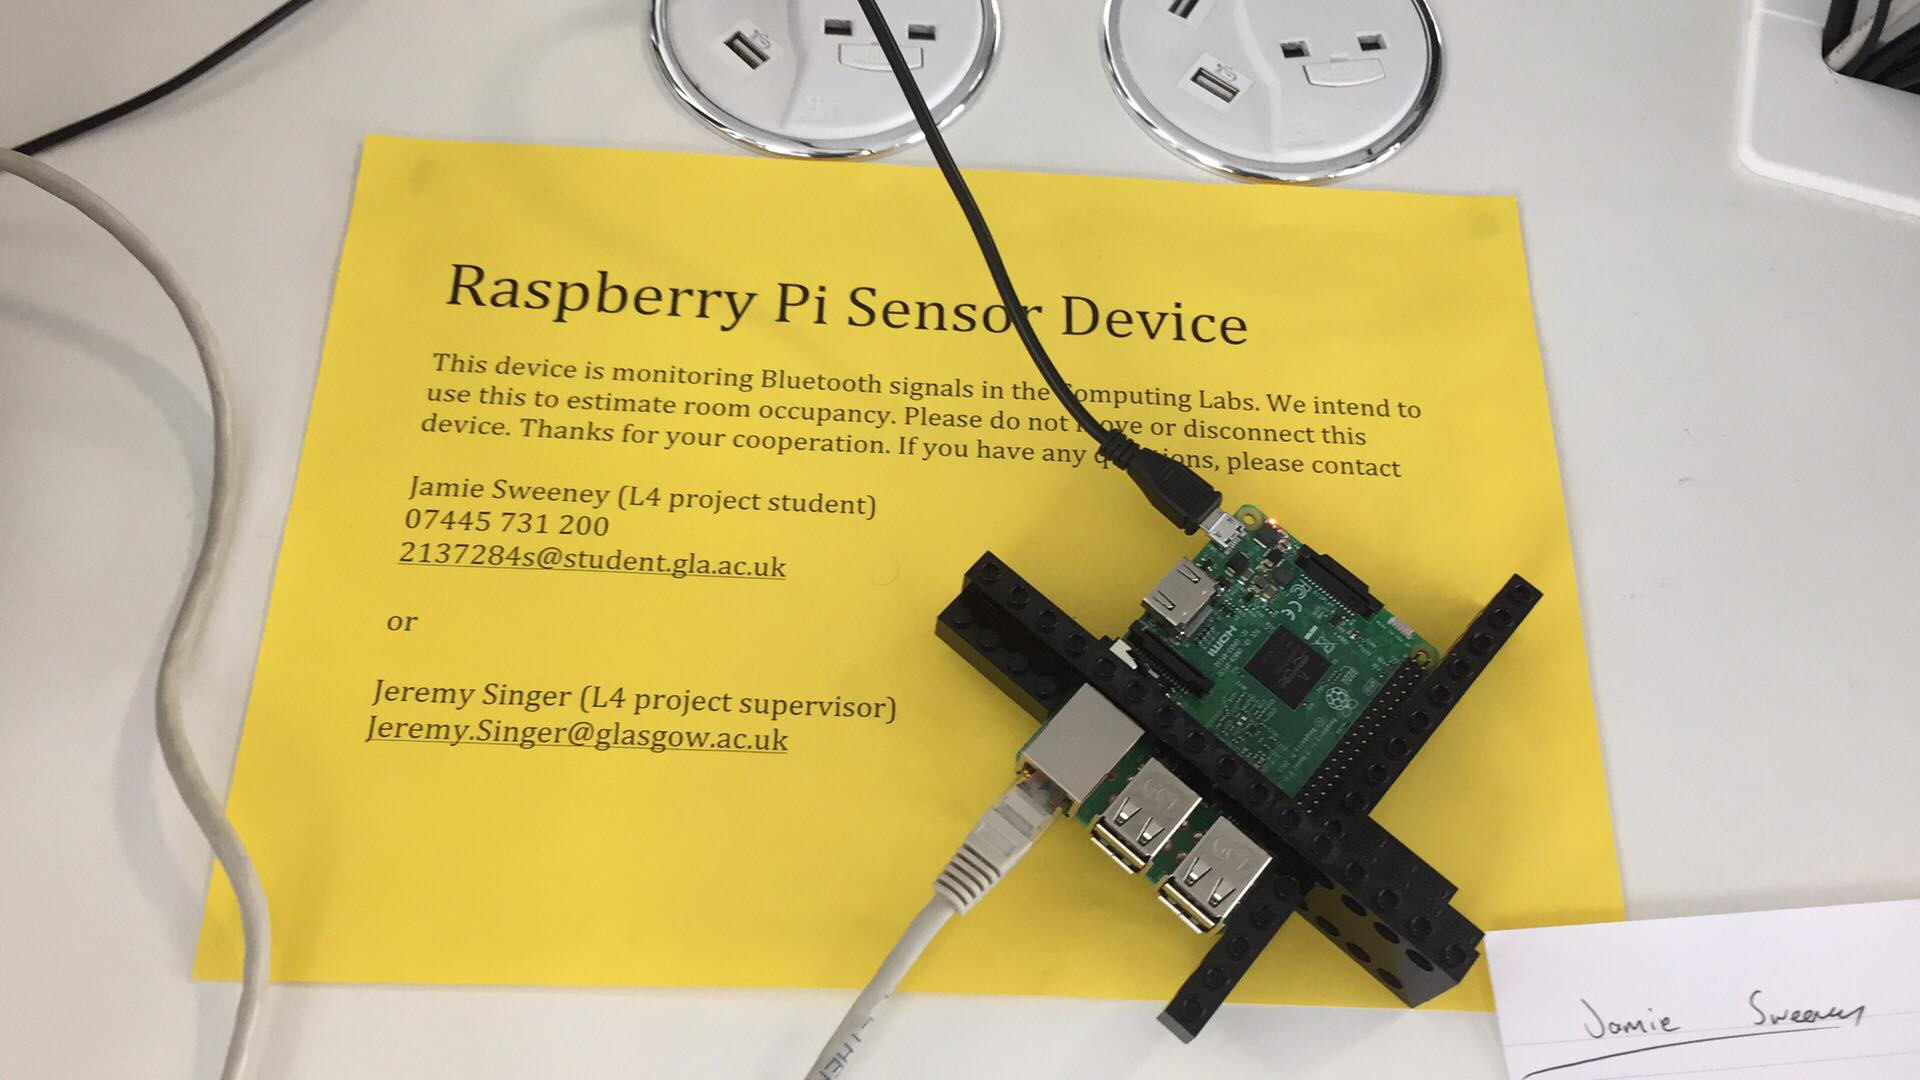
\includegraphics[width=\textwidth]{testrpi}
\caption{The production evaluation setup in BO720.}
\label{fig:testrpi}
\end{figure}

Our findings are unexpected, however they provide insight into the issues associated with a use in a production environment that were not uncovered during the first stage of evaluation. Most notably we found that Bluetooth Low Energy devices detection made up around 90-100\% of the total devices, with standard Bluetooth barely ever being detected. The 3rd year laboratory (BO720) sensor box seemed to produce relatively stable reports, albeit with several occurances of zero devices being reported, Figure \ref{fig:bo720devices} shows the reported devices against the recorded number of people in the labaratory. In comparison, the 1st year laboratory BO715 smart sensor boxes reports were highly inconsistent, we found that the number of devices would frequently drop to zero suddenly and go back to normal sudden. We are still not sure what the cause of this error is, my suspicion is that multiple instances of the reporter scripts were running on the same machine and one had acess to the resources, while another did not. However to mitigate this we proceed with evaluation using only the reports from BO720. Figure \ref{fig:bo720devices} shows the number of reported devices and the number of people counted at that time.

\begin{figure}
\centering
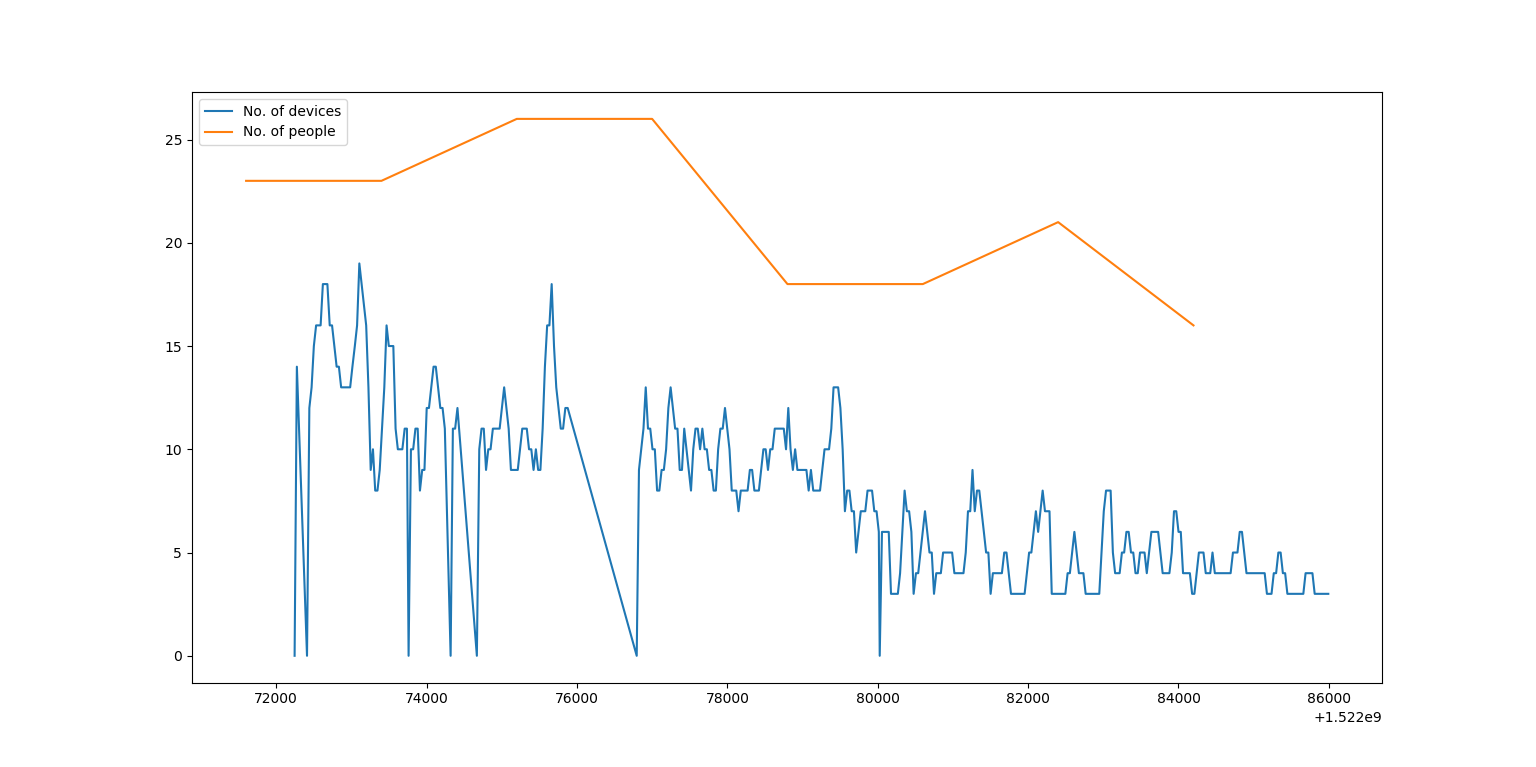
\includegraphics[width=\textwidth]{bo720devices}
\caption{BO720 reports against people counted. 26/03/2018  13:30-17:00}
\label{fig:bo720devices}
\end{figure}


\begin{figure}
\centering
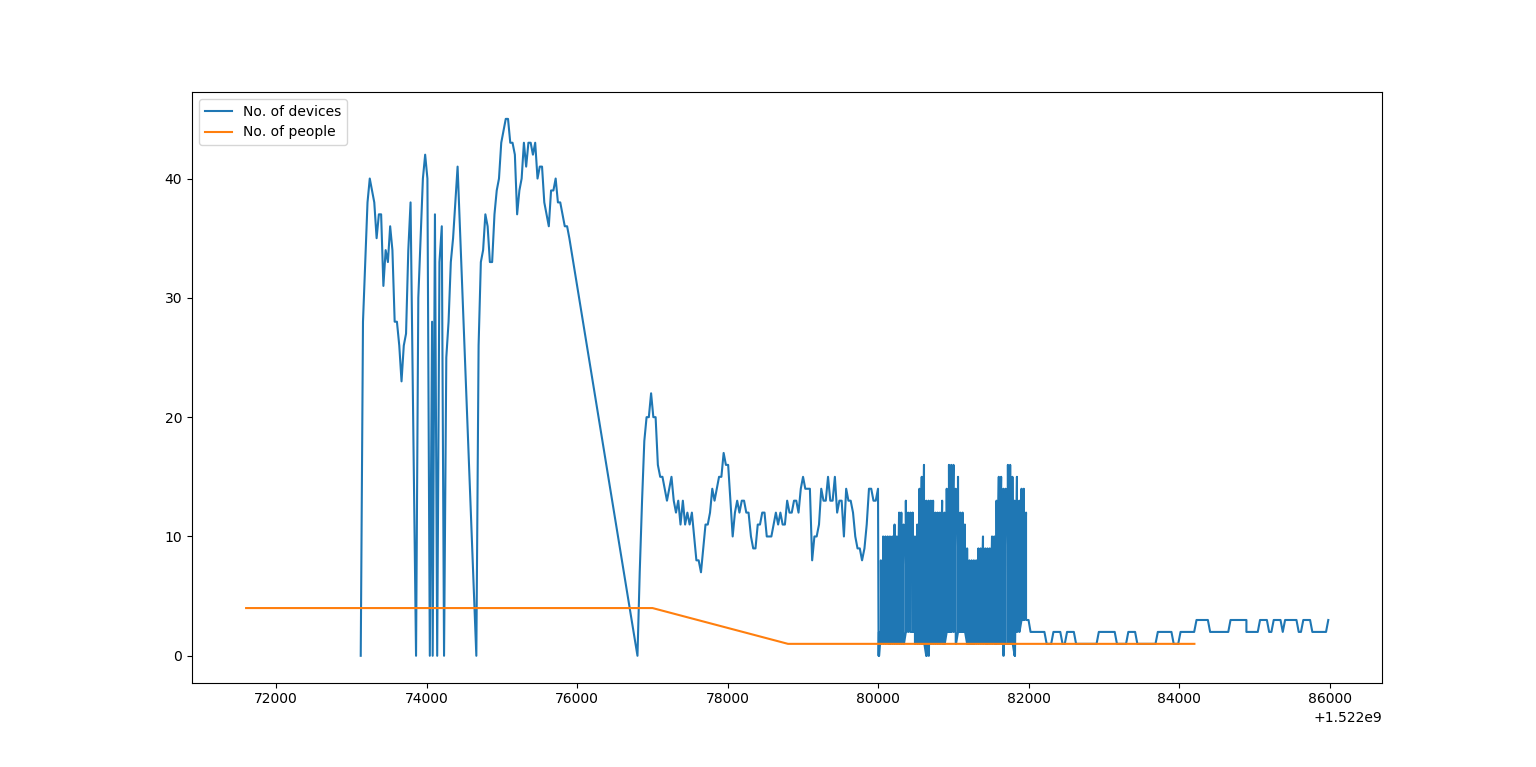
\includegraphics[width=\linewidth]{bo715devices}
\caption{BO715 reports against people counted. 26/03/2018  13:30-17:00}
\label{fig:bo715devices}
\end{figure}




\subsection{Non-functional Evaluation}
To fully evaluate the smart sensor boxes, we also evaluate the status of each non-functional requirement set out in the requirements chapter.

\begin{itemize}	
  \item Price - We calculate the standard price of a single smart sensor box to be around £52, however purchising in bulk would reduce this cost considerably, appendix \ref{appendix:rpiprice} shows the calculations made.
  \item Data collection rate - Both BT and BTLE scans are continuous which is ideal, the image capturing however, requires some processing time. We take the average time required to take an image using 5 seperate captures, we find that the time varies very little and takes an average of 4 seconds per image, which is definetely fast enough for our needs. 
  \item Maintenance required - During the production environment tests, we found that errors in the scanning processes would crash that scan, and the reporter must be manually restarted in order to restart the scanning. However the code could be modified slightly to log any error to file and attempt and automatic restart.
\end{itemize}




\section{Sesor data processing}

We perform a set of manual tests to gain an evaluation of the post processing algorithms. Tables \ref{table:scanproc} and \ref{table:imgproc} detail the manual tests performed, we find that the algorithms are mostly sufficient, however there is several oppurtunities for furthur improvements. Additionally we encountered some limitations on the system that were unavoidable as far as my knowledge.
\begin{table}
\begin{tabularx}{\textwidth}{|X|X|X|X|}
\hline
\textbf{Sub-requirement} & \textbf{Test} & \textbf{Result} & \textbf{Status}\tabularnewline
\hline
Logging & Manually compare standard output with log files. &  We find that devices are being correctly logged. & Adequate. \\
\hline 
Anonymisation of addresses & Monitor output of scan with anonymisation set as true. & Device addresses are sucessfully one-way hashed, hashing the same address produces the same result. & Adequate. \\
\hline
Collation of results & Monitor output of both threads, and of parent thread. & Devices are merged and parent output contains all devices found. & Adequate.\\
\hline
Duplicate removal & Monitor output of both threads, and of parent thread. & We find that when devices broadcast an anonymous address or respond to both Bluetooth and BTLE scans with different addresses, there is no way to merge the discoveries as they appear to be seperate devices. & Limitations. \\
\hline
Keeping results & Output is monitored with conrolled devices. & Devices data persists for the required amount of time and disappears afterwards. &  Adequate.\\ 
\hline
Smoothing results  & Manual calculations compared to post-processing standard output. & Device RSSI smoothes according to the weighted average definition. However the weightings could potentially be optimised for more accurate readings. & Possible improvements.\\
\hline
\end{tabularx}
\caption{BT and BTLE device processing test findings.}
\label{table:scanproc}
\end{table}
\begin{table}
\begin{tabularx}{\textwidth}{|X|X|X|X|}
\hline
\textbf{Sub-requirement} & \textbf{Test} & \textbf{Result} & \textbf{Status}\tabularnewline
\hline
Logging & Verify that any captured or processed images are saved to file. &  We find that all images are being correctly logged. & Adequate. \\
\hline 
Object recognition & Basic test with test image set and home-use, manually comparing bounding boxes with actual object in the image. & We find that there are many situations where people are not recognised e.g occlusion from other objects or bad angles. We could continue to train the object recognition model to obtain as accurate results as possible. & Possible improvements. \\
\hline
Parsing & Monitor output of object detection , and of parsing thread. & As expected, this is a simple parsing operation and has no issues. & Adequate.\\
\hline
Smoothing results  & Manual calculations compared to post-processing standard output. & The number of people smooths accordingly, however the weightings could potentially be optimised for more accurate readings. & Possible improvements.\\
\hline
\end{tabularx}
\caption{Image processing test findings.}
\label{table:imgproc}
\end{table}

As before, we evaluate the status of each non-functional requirement.

\begin{itemize}	
  \item Data processing speed - Since devices are loaded into the output object in virtually real-time, we must only consider the image post processing. We found that over 5 cases, the average time taken to post-process the image was 10 seconds.
  \item Data processing intensity  - We find the same is true with process intensity, the device processing is negligible, compared to the image processing which is very processer intensive, however I believe we have one of the best suited YOLO implementations and the nature of image processing tasks is unavoidable.
\end{itemize}



\section{Reports}

Additionally we perform a set of manual tests on the reporter script and discover some minor issues. The problems are relatively easy to fix, and would not be an issue if discovered sooner, this is an example of where unit integrated testing would have been useful. Table \ref{table:evalreport} gives the detaills. 
\begin{table}
\begin{tabularx}{\textwidth}{|X|X|X|X|}
\hline
\textbf{Sub-requirement} & \textbf{Test} & \textbf{Result} & \textbf{Status}\tabularnewline
\hline
Collection of post-process state  & Verify that any captured or processed images are saved to file. &  We find that all images are being correctly logged. & Adequate. \\
\hline 
Reporting & Verify on sever side that reports are being recieved and have correct structure. & We find that reports that have no associated camera, give people = 0 instead of people = null. Additionally server side errors i.e 500 Server Error, will crash the reporter script upon response. & Minor issues. \\
\hline
Logging & Monitor output of reporter script, and compare to log file. & We find that log files match correctly. & Adequate.\\
\hline
\end{tabularx}
\caption{Report manual test details.}
\label{table:evalreport}
\end{table}

The non-functional requirements are achieved for the most part, we find that since the reporter algorithm is run as a seperate process it does not suffer delay from data collection/processing. As a result, reports are accurate to the time schedule even in cases where reports are required every 5 seconds or less, however a report per minute should suffice. As stated, JSON encoding was used to format the report, which allows it to be easily extendible, we could further improve the structure by storing report sensor data as a dictionary within the "report" object. This would allow us to easily add and remove sensors without much change to design.

\section{Centralised Storage}

Evaluation of the centralised storage is fairly simple, we can see from Figure \ref{fig:ERdiagram} that all required data points are accounted for, along with the associated entity relationships. We also find that all non-functional requirements are satisfied through the Google Cloud SQL instance, specifically the access to the database is secured by SSL certificates and manual authorisation of IP addresses (of servers, development evironments etc.). 


\section{Estimating Occupancy}

Alongside the sensor data collection tests we evaluated the estimation model in the same environments. In the develoment environment, we found that there was not enough varience in occupancy or sensor readings to give a indication of real life performance. To evaluate the functional requirements before deploying, we populate the database with fake reports containing random integers. We find that the locally hosted flask application can sucessfully receive occupancy readings from admin users and then use those readings in combination with report data to generate training data. Since our choice of regression algorithm supports partially training (training multiple times), the model can be continually trained with new data. We also confirmed that multiple smart sensor boxes in the same area could be used to give an average prediction, however in retrospect it may have been more useful to take a sum of the predictions, which would make the system more scaleable to large rooms.

At first we used 2 rooms to train the model, however as we have shown in the sensor data collection evaluation section, the device scanner results were extremely different for each room. We decided that a better design choice would be to have seperate models for each room, or group the rooms and assign models for each group. This would require significant code change and was not feasible for implementation at this stage. In order to get a better understanding of how the desired system would perform, we decided to continue training the model using only the report data from BO720. 

PREDICTION / OCCUPANCY GRAPH HERE


\section{Data Serving}

The HTTP API is one of the main components that would have benifited from test cases, manual tests were performed on the public API and several small issues were uncovered. The admin API was tested through the use of the admin interface panel, however more thourough testing could be done on the API endpoints themselved as this may uncovered bugs that could arise from automated admin API calls. However since the system performs validation on admin API requests client-side (JavaScript), this will not be an immediate issue. Functional evaluation of the user interface goes well, with only a few minor issues discovered, however this is to be expected as the user interface has relatively little functionality. Table \ref{table:evaldata} gives the details of evaluation. 

We also assess the usability of the interface by performing a user experience questionnaire for both the public and admin GUI. Since the target audience of the system is mostly students, we will use students to evaluate the user experience. Our test subjects are split into 2 groups of 3 users each, based on experience with computer science. The group more familiar with computers are used to evaluate the admin GUI and conversely the less familiar group are used to evaluate the public GUI. Users are asked to explore the relevant interface and answer the following questions:

\begin{enumerate}	
  \item "How would you rate the usability (how easy it was to perform desired actions) from 1-10?"
  \item "How would you the aesthetics of the site from 1-10?"
  \item "How would you the speed/delay experienced when using site from 1-10?"
  \item "What additional comments do you have?"
\end{enumerate}

Figure \ref{fig:userrev} shows the results for the public group, results were overall positive, with all participants noting the response time. Additionally several great suggestions were made that could be acted on given more time:
\begin{itemize}	
  \item One user felt that the help page could be improved by making it more simple, specifically omitting the part about the 'HTTP API' which was generally confusing. This could be resolved by splitting the help section into two parts, one for basic users, and one for API specifics.
  \item Another user suggesting font changes to make the website stand out more.
  \item Another suggestion was adding labels to buttons on the building/floor/room page so that it was more clear that the user should click the floors/rooms etc.
  \item Finally, it was suggested that a legend should be added to the help page, showing the range of occupancy and the associated colours, as this was not immediately clear to the user.
\end{itemize}
	
\begin{figure}
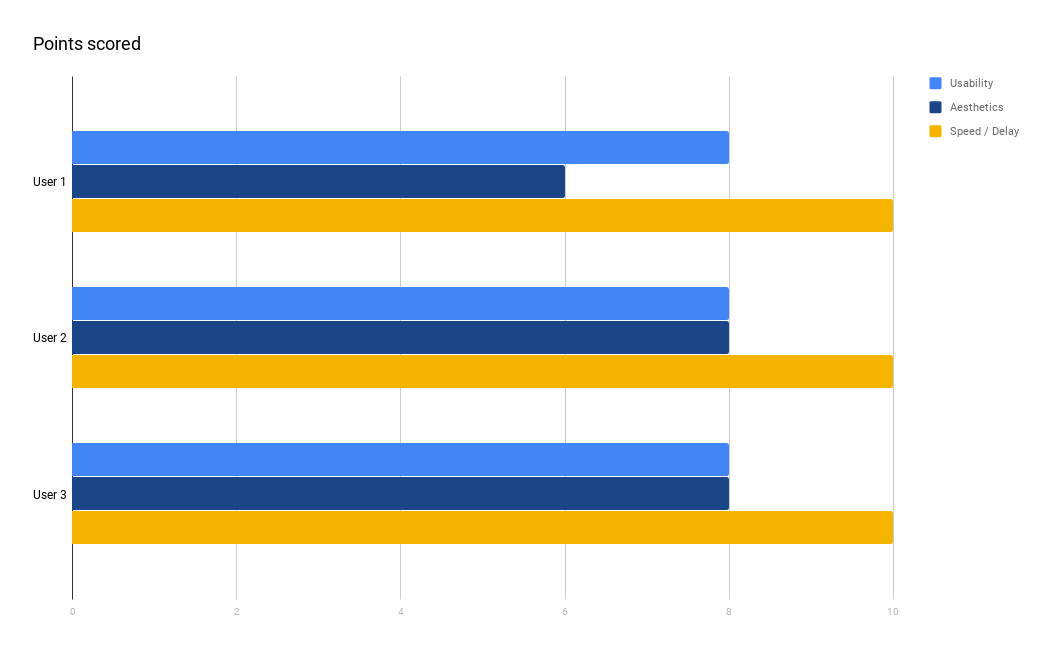
\includegraphics[width=\textwidth]{userrev}
\caption{Public user interface review.}
\label{fig:userrev}
\end{figure}

Figure \ref{fig:adminrev} shows the results for the admin group, which were slightly worse than the public interface however still good overall. There were a couple of key issues that were the main cause of most missing points:
\begin{itemize}	
  \item Datetime selector for the 'add new reading' was not very user friendly, it was suggested that we attempt to create the datetime popup selector on click of the time input field, instead of requiring the user to press a icon inside the input field.
  \item When adding new data, the application would reload and fail to expand previously expanded tables, so users would have to extend an entity and rescroll all the way to the bottom of the page after every change. Although this does not impair functionality, it has a negative effect on the user experience and could be easily fixed.
  \item Another potential improvement was to combine the building, floor, room and rpi table into one table. This sounds promisisng however would require some careful design before being able to fit all the data in the table in a user friendly way.


\end{itemize}
	
\begin{figure}
\centering
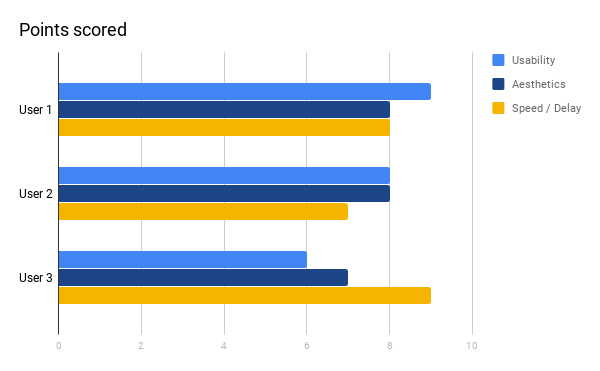
\includegraphics[width=\textwidth]{adminrev}
\caption{Admin panel user interface review.}
\label{fig:adminrev}
\end{figure}




\begin{table}
\begin{tabularx}{\textwidth}{|X|X|X|X|}
\hline
\textbf{Sub-requirement} & \textbf{Test} & \textbf{Result} & \textbf{Status}\tabularnewline
\hline
Public API & Manual testing of public api calls to localhost. & Several issues were uncovered during testing, most severe bug discovered was 500 Server Errors when requesting non-existant buildings, floors etc. & Moderate issues. \\
\hline
Admin API & Manual testing through web interface & No errors occurred when using the API through the user interface. & No issues discovered. \\
\hline
Public user interface & Manual testing of required functions & One small bug found, floors with no predictions would give a "NULL" total instead of "???". & Small issue. \\
\hline
Admin user interface & Manual testing of required functions & We found that sometimes refreshing the page was necessary to update the page with new changes. However all functions perform as expected. & Possible improvements. \\
\hline
\end{tabularx}
\caption{Functional evaluation details of data serving component.}
\label{table:evaldata}
\end{table}


%==============================================================================
%==============================================================================
%==============================================================================
\chapter{Conclusion}
\section{Summary}
\section{Future Work}
\section{Reflection}











%==============================================================================
%==============================================================================
%==============================================================================
%==Images and algorithms














%==============================================================================
%==============================================================================
%==============================================================================
%%%%%%%%%%%%%%%%
%              %
%  APPENDICES  %
%              %
%%%%%%%%%%%%%%%%
\begin{appendices}
\end{appendices}

%%%%%%%%%%%%%%%%%%%%
%   BIBLIOGRAPHY   %
%%%%%%%%%%%%%%%%%%%%

\bibliographystyle{plain}
\bibliography{bib}

\end{document}
